\documentclass{beamer}
\usepackage[utf8]{inputenc}
\usepackage[francais]{babel}
\usepackage{amsmath}
\usepackage[squaren,Gray]{SIunits}
\usepackage{numprint}
\usepackage{amsfonts}
\usepackage{amssymb}
\usepackage{graphicx}
\usepackage{mathtools}
\usepackage{mhchem}
\usepackage{hyperref}
\usepackage{varwidth}
\usetheme{Warsaw}
\title{Présentation Tâche 1:\\ bilans de matière et d’énergie du procédé
}
\author{Groupe 1246}
\institute{École Polytechnique de Louvain}
\date{}
\begin{document}

\begin{frame}
\titlepage
\end{frame}


\begin{frame}
\frametitle{Bilan de matière}
\framesubtitle{avec un exemple de sous-titre}

\begin{itemize}
	\item $F_{\ce{CH4}}$ le débit molaire de \ce{CH4}.
	\item $F_{\ce{H2O}}$ le débit molaire d'\ce{H2O}.
	\item $\xi_1$ le degré d'avancement de la réaction à l'équilibre (1).
	\item $\xi_2$ le degré d'avancement de la réaction à l'équilibre (2).
	\item $F_{\text{air}}$ le débit molaire d'air.
\end{itemize}

\end{frame}




\begin{frame}
\frametitle{Bilan de matière}
\framesubtitle{avec un exemple de sous-titre}

\begin{itemize}
	\item Réaction 1 du reformage primaire:\\
	$\ce{CH_4} + \ce{H_{2}O} \rightleftharpoons \ce{3H_2} + \ce{CO}$
	\item Réaction 2 du reformage primaire:\\
	$\ce{CO} + \ce{H_{2}O} \rightleftharpoons \ce{H_2} + \ce{CO_2}$ 
	\item Réaction du reformage secondaire:\\
	$\ce{2CH_4} + \ce{O_2} \rightarrow \ce{2CO} + \ce{4H_2}$ 
	\item Réaction dans les réacteurs Water-Gas-Shift:\\
	$\ce{CO} + \ce{H_{2}O} \rightarrow \ce{H_2} + \ce{CO_2}$ 
	\item Synthèse d'ammoniac:\\
	$\ce{N_2} + \ce{3H_2} \rightarrow \ce{2NH_3}$\\
	(Réaction incomplète en réalité, $\ce{N_2} + \ce{3H_2} \rightleftharpoons \ce{2NH_3}$ mais la réaction globale peut être considérée comme complète grâce au "recyclage")
\end{itemize}

\end{frame}



\begin{frame}
\frametitle{Bilan de matière}
\framesubtitle{avec un exemple de sous-titre}

En écrivant des tableaux d'avancement pour toutes ces réactions et en injectant dans les équations obtenues les débits initiaux, nous sommes en mesure d'obtenir des expressions pour les constantes d'équilibre $K_1(T)$ et $K_2(T)$.

Avec \textsc{Matlab} nous pouvons également calculer la valeur théorique de ces constantes d'équilibre en fonction de la température en posant la pression du reformeur primaire à \unit{30}{\bbar}.

\end{frame}



\begin{frame}
\frametitle{Bilan d'énergie}
\framesubtitle{Réacteur de reformage primaire}



$$\Delta H\degree_{Reaction1}(T)=3 \cdot \Delta H\degree_{H_{2(g)}}(T) + \Delta H\degree_{CO_{(g)}}(T) ~- \\ ~~~~~~~~~~~~~~~~~~~~~~~~~~~~~~~~~~~~~~~~~~
\lbrack\Delta H\degree_{CH_{4(g)}}(T) + \Delta H\degree_{H_{2}O_{(g)}}(T)\rbrack$$


$$\Delta H\degree_{Reaction2}(T)=$$


$$\Delta H\degree_{Reacteur}(T)=\xi_1\cdot\Delta H\degree_{Reaction1,m}(T)+\xi_2\cdot\Delta H\degree_{Reaction2,m}(T)$$

\end{frame}



\begin{frame}
\frametitle{Bilan d'énergie}
\framesubtitle{Four}

$$\Delta H\degree_{Four,m} = 2\cdot \Delta H\degree_{H_{2}O_{(g)}} + \Delta H\degree_{CO_{2(g)}}
- \left(\Delta H\degree_{CH_{4(g)}} + 2\cdot \Delta H\degree_{O_{2(g)}}\right)$$


\end{frame}


\begin{frame}
\frametitle{Bilan d'énergie}
\framesubtitle{Quantité de \ce{CH_4}}

$$\text{Quantité de \ce{CH_4}} = \dfrac{\Delta H_{Reacteur}}{\Delta H_{Four,m}}$$


\end{frame}



\begin{frame}
\frametitle{Analyse paramétrique}
\framesubtitle{Quantité de \ce{CH_4}}

\begin{figure}[ht!]
\centering
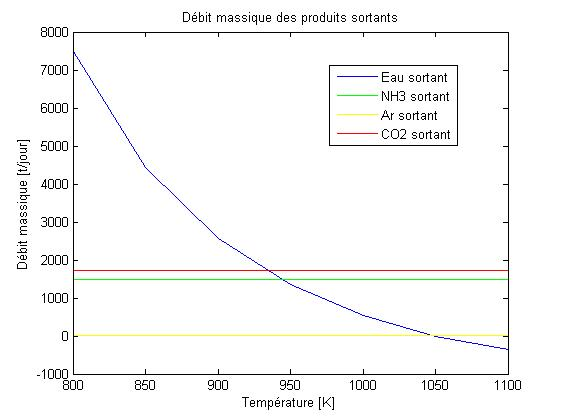
\includegraphics[scale=0.4]{produits.jpg}
\end{figure}


\end{frame}



\end{document}
